\documentclass[xcolor=dvipsnames]{beamer}
\usetheme{default}

\definecolor{clrfg}{RGB}{0,0,0}
\definecolor{clrfg2}{RGB}{0,103,198}
\definecolor{clrbg}{RGB}{255,255,255}
\definecolor{clrbg2}{RGB}{230,230,230}

\setbeamercolor{alerted text}{fg=clrfg2}
\setbeamercolor{background canvas}{bg=clrbg}
\setbeamercolor{block title}{bg=clrbg2, fg=clrfg2}
\setbeamercolor{frametitle}{fg=clrbg}
\setbeamercolor{item projected}{fg=clrbg}
\setbeamercolor{sidebar}{bg=clrbg}
\setbeamercolor{sidebar}{parent=palette primary}
\setbeamercolor{structure}{bg=clrfg2, fg=clrfg2}
\setbeamercolor{subsection in sidebar}{fg=clrbg}
\setbeamercolor{subsection in sidebar shaded}{fg=clrbg}
\setbeamercolor{title}{fg=clrbg}
\setbeamercolor{titlelike}{fg=clrbg}

\usepackage[czech]{babel}
\usepackage[utf8]{inputenc}
\usepackage{graphicx}
\graphicspath{{..//thesis//figures//}}
\setbeamertemplate{navigation symbols}{} 
\titlegraphic{\includegraphics[width=0.22\paperwidth]{ctu.pdf}}
\title{Optimalizace rozmístění obdelníkových útvarů \\pomocí evolučních algoritmů}
\author{Vojtěch Hordějčuk}
\institute{FEL ČVUT}
\date{\today}

\begin{document}

\frame {
  \titlepage
}

%===============================================================================
\section{Úvod}
%===============================================================================

\frame {
	\frametitle{Úvod}
	
	\begin{block}{Řešený problém}
	\begin{itemize}
	\item{optimální rozmístění obdélníků na plochu}
	\item{NP-těžký optimalizační problém}
	\item{hlavní motivace = {\bf ušetřit}}
	\end{itemize}
	\end{block}
	
	\begin{block}{Využití v praxi}
	\begin{itemize}
	\item{VLSI floorplanning}% {\tiny(zvýšení maximální frekvence, zmenšení plochy čipu\ldots)}}
	\item{urbanistika}% {\tiny(rozumné rozmístění veřejných budov\ldots)}}
	\item{plánování}% {\tiny(optimální alokace zdrojů v čase\ldots)}}
	\end{itemize}
	\end{block}
}

\frame {
	\frametitle{Cíle práce}
	\begin{enumerate}
	\item{zvolit vhodnou a efektivní {\bf reprezentaci}}
	\item{navrhnout evoluční {\bf algoritmus}}
	\item{provést {\bf benchmarky} (GSRC, MCNC)}
	\item{{\bf výsledky} vyhodnotit a porovnat}
	\end{enumerate}
}

%===============================================================================
\section{Jiná řešení}
%===============================================================================

\frame {
	\frametitle{Varianty přístupu}
	
	\begin{block}{Možné reprezentace}
	\begin{itemize}
	\item{{\bf Slicing Tree} -- binární strom, slicing}
	\item{{\bf sekvenční páry} -- uspořádaná dvojice permutací, non-slicing}
	\item{{\bf Corner Block List} -- uspořádaná trojice, non-slicing}
	\item{{\bf O-Tree} -- obecný strom, non-slicing}
	\item{{\bf B*-Tree} -- binární strom, non-slicing}
	\end{itemize}
	\end{block}
	
  \begin{block}{Používané optimalizační algoritmy}
	\begin{itemize}
	\item{deterministické (DFS, BFS)}
	\item{simulované ochlazování}
	\item{evoluční algoritmy}
	\end{itemize}
  \end{block}
}

%===============================================================================
\section{Navržené řešení}
%===============================================================================

\frame {
	\frametitle{Navržené řešení}

	B*-Tree reprezentace + Algoritmus POEMS \footnote{http://code.google.com/p/vh-master-thesis/}

	\begin{block}{B*-Tree reprezentace}
	\begin{itemize}
	\item{binární strom}
	\item{levý potomek - umístit {\bf vedle}}
	\item{pravý potomek - umístit {\bf nad}}
	\end{itemize}
	\end{block}

  \begin{block}{Algoritmus POEMS}
  
  \begin{itemize}
  \item{počáteční řešení (prototyp) $\leftarrow$ best-fit heuristika}
  \item{iterativní hledání nejlepší modifikace prototypu}
  \item{modifikace prototypu $\leftarrow$ sekvence definovaných akcí}
  \item{optimalizace sekvencí $\leftarrow$ genetický algoritmus}
  \end{itemize}
  \end{block}
 
}

\frame {
	\frametitle{B*-Tree reprezentace (příklad) \footnote{kořen = vlevo nahoře, červená = levá, modrá = pravá}}

	\begin{center}
	\includegraphics[width=0.82\textwidth]{btreebig1.pdf}	
	\end{center}

}

\frame {
	\frametitle{Algoritmus POEMS}

	\begin{itemize}
	\item{iterativní algoritmus}
	\item{lokální prohledávání pomocí evolučního algoritmu}
	\item{počáteční řešení (prototyp) náhodně či heuristikou}
	\item{modifikace prototypu sekvencemi elementárních akcí}
		\begin{enumerate}
		\item{{\bf ROTATE}}
		\item{{\bf MOVE NODE, MOVE VALUE, FLIP, MIRROR}}
		\item{{\bf HANG NODE}}
		\end{enumerate}
	\item{evoluční algoritmus mění akce a parametry}
	\end{itemize}

	%\begin{center}
	%\includegraphics[height=.3\textheight]{ami49evolution.pdf}
	%\end{center}
}

\frame {
	\frametitle{Algoritmus POEMS}

	\begin{center}
	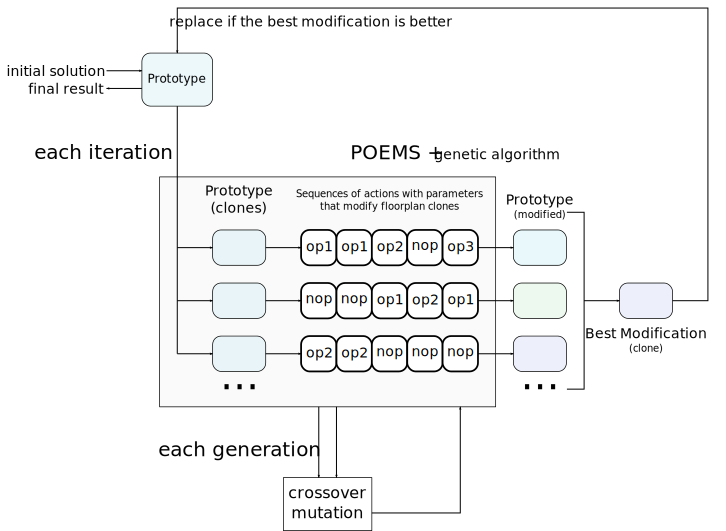
\includegraphics[height=0.73\paperheight]{algorithm.pdf}
	\end{center}
}

%===============================================================================
\section{Experimenty}
%===============================================================================

\frame {
	\frametitle{Experimenty: Data a konfigurace}
	
	\begin{block}{Benchmarky}
	\begin{itemize}
	\item{MCNC (9 -- 49 bloků)}
	\item{GSRC (10 -- stovky bloků)}
	\end{itemize} 
	\end{block}

	\begin{block}{Algoritmy}
	\begin{itemize}
	\item{{\bf B*-Tree/POEMS} - navržený algoritmus, 50,000 iterací}
	\item{{\bf CompaSS} - O-Tree, Slicing Tree, větve a hranice}
	\item{{\bf B*-Tree/I} - iterativní algoritmus}
	\item{{\bf B*-Tree/SA} - simulované ochlazování}
	\end{itemize} 
	\end{block}
}

\frame {
	\frametitle{Experimenty: Výsledky}

  \begin{center}
  \small\begin{tabular}{|r|c|c|c|c|c|}
  \hline
   & B*-Tree/POEMS & CompaSS & B*-Tree/I & B*-Tree/SA \\
  \hline
  \hline
  apte & 0.78\% (969 s) & 0.78\% (0 s) & {\bf 0.77\%} (7 s) & 1.59\% (2 s) \\
  \hline
  xerox & {\bf 2.30\%} (902 s) & 3.45\% (16 s) & 2.48\% (25 s) & 3.85\% (5 s) \\
  \hline
  hp & 3.88\% (1,927 s) & 2.28\% (3 s) & {\bf 1.35\%} (55 s) & 4.47\% (20 s) \\
  \hline
  n100 & {\bf 1.98\%} (4,826 s) & 7.32\% (4 s) & N/A & N/A \\
  \hline
  n200 & {\bf 3.68\%} (8,408 s) & 6.48\% (10 s) & N/A & N/A \\
  \hline
  \end{tabular}
  \end{center}

	\hfill

	\begin{itemize}
	\item{průměrné hodnoty (10 a více běhů)}
	\item{{\bf většínou lepší výsledky než konkurence}}
	\item{cenou za kvalitu je delší výpočet}
	\end{itemize}
}

%===============================================================================
\section{Shrnutí}
%===============================================================================


\frame {
	\frametitle{Shrnutí}

	\begin{itemize}
	\item{navzdory nedostatečnému popisu v literatuře navržena {\bf efektivní} a {\bf úsporná} reprezentace}
	\item{dosažené výsledky ve kvalitě zhruba {\bf dvojnásobně překonávají} slicing reprezentaci}
	\item{naměřené výsledky jsou minimálně srovnatelné a {\bf často lepší} než ostatní porovnávané algoritmy}
	\item{připravujeme {\bf článek} do časopisu}
	\end{itemize}
}

%===============================================================================
\section{Animace (n300)}
%===============================================================================

\frame {
	\frametitle{Animace (n300) -- 1 / 20}
	\begin{center}
	\includegraphics[height=0.7\paperheight]{n300/0.pdf}
	\end{center}
}

\frame {
	\frametitle{Animace (n300) -- 2 / 20}
	\begin{center}
	\includegraphics[height=0.7\paperheight]{n300/4.pdf}
	\end{center}
}

\frame {
	\frametitle{Animace (n300) -- 3 / 20}
	\begin{center}
	\includegraphics[height=0.7\paperheight]{n300/8.pdf}
	\end{center}
}

\frame {
	\frametitle{Animace (n300) -- 4 / 20}
	\begin{center}
	\includegraphics[height=0.7\paperheight]{n300/12.pdf}
	\end{center}
}

\frame {
	\frametitle{Animace (n300) -- 5 / 20}
	\begin{center}
	\includegraphics[height=0.7\paperheight]{n300/16.pdf}
	\end{center}
}

\frame {
	\frametitle{Animace (n300) -- 6 / 20}
	\begin{center}
	\includegraphics[height=0.7\paperheight]{n300/20.pdf}
	\end{center}
}

\frame {
	\frametitle{Animace (n300) -- 7 / 20}
	\begin{center}
	\includegraphics[height=0.7\paperheight]{n300/24.pdf}
	\end{center}
}

\frame {
	\frametitle{Animace (n300) -- 8 / 20}
	\begin{center}
	\includegraphics[height=0.7\paperheight]{n300/28.pdf}
	\end{center}
}

\frame {
	\frametitle{Animace (n300) -- 9 / 20}
	\begin{center}
	\includegraphics[height=0.7\paperheight]{n300/32.pdf}
	\end{center}
}

\frame {
	\frametitle{Animace (n300) -- 10 / 20}
	\begin{center}
	\includegraphics[height=0.7\paperheight]{n300/38.pdf}
	\end{center}
}

\frame {
	\frametitle{Animace (n300) -- 11 / 20}
	\begin{center}
	\includegraphics[height=0.7\paperheight]{n300/42.pdf}
	\end{center}
}

\frame {
	\frametitle{Animace (n300) -- 12 / 20}
	\begin{center}
	\includegraphics[height=0.7\paperheight]{n300/45.pdf}
	\end{center}
}

\frame {
	\frametitle{Animace (n300) -- 13 / 20}
	\begin{center}
	\includegraphics[height=0.7\paperheight]{n300/48.pdf}
	\end{center}
}

\frame {
	\frametitle{Animace (n300) -- 14 / 20}
	\begin{center}
	\includegraphics[height=0.7\paperheight]{n300/50.pdf}
	\end{center}
}

\frame {
	\frametitle{Animace (n300) -- 15 / 20}
	\begin{center}
	\includegraphics[height=0.7\paperheight]{n300/53.pdf}
	\end{center}
}

\frame {
	\frametitle{Animace (n300) -- 16 / 20}
	\begin{center}
	\includegraphics[height=0.7\paperheight]{n300/56.pdf}
	\end{center}
}

\frame {
	\frametitle{Animace (n300) -- 17 / 20}
	\begin{center}
	\includegraphics[height=0.7\paperheight]{n300/59.pdf}
	\end{center}
}

\frame {
	\frametitle{Animace (n300) -- 18 / 20}
	\begin{center}
	\includegraphics[height=0.7\paperheight]{n300/61.pdf}
	\end{center}
}

\frame {
	\frametitle{Animace (n300) -- 19 / 20}
	\begin{center}
	\includegraphics[height=0.7\paperheight]{n300/63.pdf}
	\end{center}
}

\frame {
	\frametitle{Animace (n300) -- 20 / 20}
	\begin{center}
	\includegraphics[height=0.7\paperheight]{n300/66.pdf}
	\end{center}
}

\end{document}
